% Options for packages loaded elsewhere
\PassOptionsToPackage{unicode}{hyperref}
\PassOptionsToPackage{hyphens}{url}
%
\documentclass[
  english,
  man]{apa6}
\usepackage{amsmath,amssymb}
\usepackage{lmodern}
\usepackage{ifxetex,ifluatex}
\ifnum 0\ifxetex 1\fi\ifluatex 1\fi=0 % if pdftex
  \usepackage[T1]{fontenc}
  \usepackage[utf8]{inputenc}
  \usepackage{textcomp} % provide euro and other symbols
\else % if luatex or xetex
  \usepackage{unicode-math}
  \defaultfontfeatures{Scale=MatchLowercase}
  \defaultfontfeatures[\rmfamily]{Ligatures=TeX,Scale=1}
\fi
% Use upquote if available, for straight quotes in verbatim environments
\IfFileExists{upquote.sty}{\usepackage{upquote}}{}
\IfFileExists{microtype.sty}{% use microtype if available
  \usepackage[]{microtype}
  \UseMicrotypeSet[protrusion]{basicmath} % disable protrusion for tt fonts
}{}
\makeatletter
\@ifundefined{KOMAClassName}{% if non-KOMA class
  \IfFileExists{parskip.sty}{%
    \usepackage{parskip}
  }{% else
    \setlength{\parindent}{0pt}
    \setlength{\parskip}{6pt plus 2pt minus 1pt}}
}{% if KOMA class
  \KOMAoptions{parskip=half}}
\makeatother
\usepackage{xcolor}
\IfFileExists{xurl.sty}{\usepackage{xurl}}{} % add URL line breaks if available
\IfFileExists{bookmark.sty}{\usepackage{bookmark}}{\usepackage{hyperref}}
\hypersetup{
  pdftitle={Light Exposure Behavior Assessment (LEBA): Develop of a novel instrument to capture light exposure-related behaviours},
  pdfauthor={Mushfiqul Anwar Siraji1, Rafael Robert Lazar2, Manuel Spitschan3, \& Manuel Spitschan3},
  pdflang={en-EN},
  pdfkeywords={keywords},
  hidelinks,
  pdfcreator={LaTeX via pandoc}}
\urlstyle{same} % disable monospaced font for URLs
\usepackage{graphicx}
\makeatletter
\def\maxwidth{\ifdim\Gin@nat@width>\linewidth\linewidth\else\Gin@nat@width\fi}
\def\maxheight{\ifdim\Gin@nat@height>\textheight\textheight\else\Gin@nat@height\fi}
\makeatother
% Scale images if necessary, so that they will not overflow the page
% margins by default, and it is still possible to overwrite the defaults
% using explicit options in \includegraphics[width, height, ...]{}
\setkeys{Gin}{width=\maxwidth,height=\maxheight,keepaspectratio}
% Set default figure placement to htbp
\makeatletter
\def\fps@figure{htbp}
\makeatother
\setlength{\emergencystretch}{3em} % prevent overfull lines
\providecommand{\tightlist}{%
  \setlength{\itemsep}{0pt}\setlength{\parskip}{0pt}}
\setcounter{secnumdepth}{-\maxdimen} % remove section numbering
% Make \paragraph and \subparagraph free-standing
\ifx\paragraph\undefined\else
  \let\oldparagraph\paragraph
  \renewcommand{\paragraph}[1]{\oldparagraph{#1}\mbox{}}
\fi
\ifx\subparagraph\undefined\else
  \let\oldsubparagraph\subparagraph
  \renewcommand{\subparagraph}[1]{\oldsubparagraph{#1}\mbox{}}
\fi
% Manuscript styling
\usepackage{upgreek}
\captionsetup{font=singlespacing,justification=justified}

% Table formatting
\usepackage{longtable}
\usepackage{lscape}
% \usepackage[counterclockwise]{rotating}   % Landscape page setup for large tables
\usepackage{multirow}		% Table styling
\usepackage{tabularx}		% Control Column width
\usepackage[flushleft]{threeparttable}	% Allows for three part tables with a specified notes section
\usepackage{threeparttablex}            % Lets threeparttable work with longtable

% Create new environments so endfloat can handle them
% \newenvironment{ltable}
%   {\begin{landscape}\begin{center}\begin{threeparttable}}
%   {\end{threeparttable}\end{center}\end{landscape}}
\newenvironment{lltable}{\begin{landscape}\begin{center}\begin{ThreePartTable}}{\end{ThreePartTable}\end{center}\end{landscape}}

% Enables adjusting longtable caption width to table width
% Solution found at http://golatex.de/longtable-mit-caption-so-breit-wie-die-tabelle-t15767.html
\makeatletter
\newcommand\LastLTentrywidth{1em}
\newlength\longtablewidth
\setlength{\longtablewidth}{1in}
\newcommand{\getlongtablewidth}{\begingroup \ifcsname LT@\roman{LT@tables}\endcsname \global\longtablewidth=0pt \renewcommand{\LT@entry}[2]{\global\advance\longtablewidth by ##2\relax\gdef\LastLTentrywidth{##2}}\@nameuse{LT@\roman{LT@tables}} \fi \endgroup}

% \setlength{\parindent}{0.5in}
% \setlength{\parskip}{0pt plus 0pt minus 0pt}

% Overwrite redefinition of paragraph and subparagraph by the default LaTeX template
% See https://github.com/crsh/papaja/issues/292
\makeatletter
\renewcommand{\paragraph}{\@startsection{paragraph}{4}{\parindent}%
  {0\baselineskip \@plus 0.2ex \@minus 0.2ex}%
  {-1em}%
  {\normalfont\normalsize\bfseries\itshape\typesectitle}}

\renewcommand{\subparagraph}[1]{\@startsection{subparagraph}{5}{1em}%
  {0\baselineskip \@plus 0.2ex \@minus 0.2ex}%
  {-\z@\relax}%
  {\normalfont\normalsize\itshape\hspace{\parindent}{#1}\textit{\addperi}}{\relax}}
\makeatother

% \usepackage{etoolbox}
\makeatletter
\patchcmd{\HyOrg@maketitle}
  {\section{\normalfont\normalsize\abstractname}}
  {\section*{\normalfont\normalsize\abstractname}}
  {}{\typeout{Failed to patch abstract.}}
\patchcmd{\HyOrg@maketitle}
  {\section{\protect\normalfont{\@title}}}
  {\section*{\protect\normalfont{\@title}}}
  {}{\typeout{Failed to patch title.}}
\makeatother
\shorttitle{Title}
\keywords{keywords\newline\indent Word count: X}
\DeclareDelayedFloatFlavor{ThreePartTable}{table}
\DeclareDelayedFloatFlavor{lltable}{table}
\DeclareDelayedFloatFlavor*{longtable}{table}
\makeatletter
\renewcommand{\efloat@iwrite}[1]{\immediate\expandafter\protected@write\csname efloat@post#1\endcsname{}}
\makeatother
\usepackage{lineno}

\linenumbers
\usepackage{csquotes}
\ifxetex
  % Load polyglossia as late as possible: uses bidi with RTL langages (e.g. Hebrew, Arabic)
  \usepackage{polyglossia}
  \setmainlanguage[]{english}
\else
  \usepackage[main=english]{babel}
% get rid of language-specific shorthands (see #6817):
\let\LanguageShortHands\languageshorthands
\def\languageshorthands#1{}
\fi
\ifluatex
  \usepackage{selnolig}  % disable illegal ligatures
\fi
\newlength{\cslhangindent}
\setlength{\cslhangindent}{1.5em}
\newlength{\csllabelwidth}
\setlength{\csllabelwidth}{3em}
\newenvironment{CSLReferences}[2] % #1 hanging-ident, #2 entry spacing
 {% don't indent paragraphs
  \setlength{\parindent}{0pt}
  % turn on hanging indent if param 1 is 1
  \ifodd #1 \everypar{\setlength{\hangindent}{\cslhangindent}}\ignorespaces\fi
  % set entry spacing
  \ifnum #2 > 0
  \setlength{\parskip}{#2\baselineskip}
  \fi
 }%
 {}
\usepackage{calc}
\newcommand{\CSLBlock}[1]{#1\hfill\break}
\newcommand{\CSLLeftMargin}[1]{\parbox[t]{\csllabelwidth}{#1}}
\newcommand{\CSLRightInline}[1]{\parbox[t]{\linewidth - \csllabelwidth}{#1}\break}
\newcommand{\CSLIndent}[1]{\hspace{\cslhangindent}#1}

\title{\emph{Light Exposure Behavior Assessment (LEBA)}: Develop of a novel instrument to capture light exposure-related behaviours}
\author{Mushfiqul Anwar Siraji\textsuperscript{1}, Rafael Robert Lazar\textsuperscript{2}, Manuel Spitschan\textsuperscript{3}, \& Manuel Spitschan\textsuperscript{3}}
\date{}


\authornote{

Add complete departmental affiliations for each author here. Each new line herein must be indented, like this line.

Enter author note here.

The authors made the following contributions. Mushfiqul Anwar Siraji: Data Analysis, Writing - Original Draft Preparation, Data Visualization; Rafael Robert Lazar: Data Analysis, Writing - Original Draft Preparation, Data Visualization; Manuel Spitschan: Data Analysis, Writing - Original Draft Preparation, Data Visualization; Manuel Spitschan: Data Analysis, Writing - Original Draft Preparation, Data Visualization.

Correspondence concerning this article should be addressed to Manuel Spitschan, . E-mail:

}

\affiliation{\vspace{0.5cm}\textsuperscript{1} Department of Psychology, Jeffrey Cheah School of Medicine and Health Sciences, Monash University, Malaysia\\\textsuperscript{2} University of Basel}

\abstract{
One or two sentences providing a \textbf{basic introduction} to the field, comprehensible to a scientist in any discipline.

Two to three sentences of \textbf{more detailed background}, comprehensible to scientists in related disciplines.

One sentence clearly stating the \textbf{general problem} being addressed by this particular study.

One sentence summarizing the main result (with the words ``\textbf{here we show}'' or their equivalent).

Two or three sentences explaining what the \textbf{main result} reveals in direct comparison to what was thought to be the case previously, or how the main result adds to previous knowledge.

One or two sentences to put the results into a more \textbf{general context}.

Two or three sentences to provide a \textbf{broader perspective}, readily comprehensible to a scientist in any discipline.
}



\begin{document}
\maketitle

\hypertarget{introduction}{%
\section{Introduction}\label{introduction}}

\hypertarget{methods}{%
\section{Methods}\label{methods}}

\hypertarget{participants}{%
\subsection{Participants}\label{participants}}

This line is just a test for pushing in the github repo.

\hypertarget{material}{%
\subsection{Material}\label{material}}

\begin{figure}

{\centering 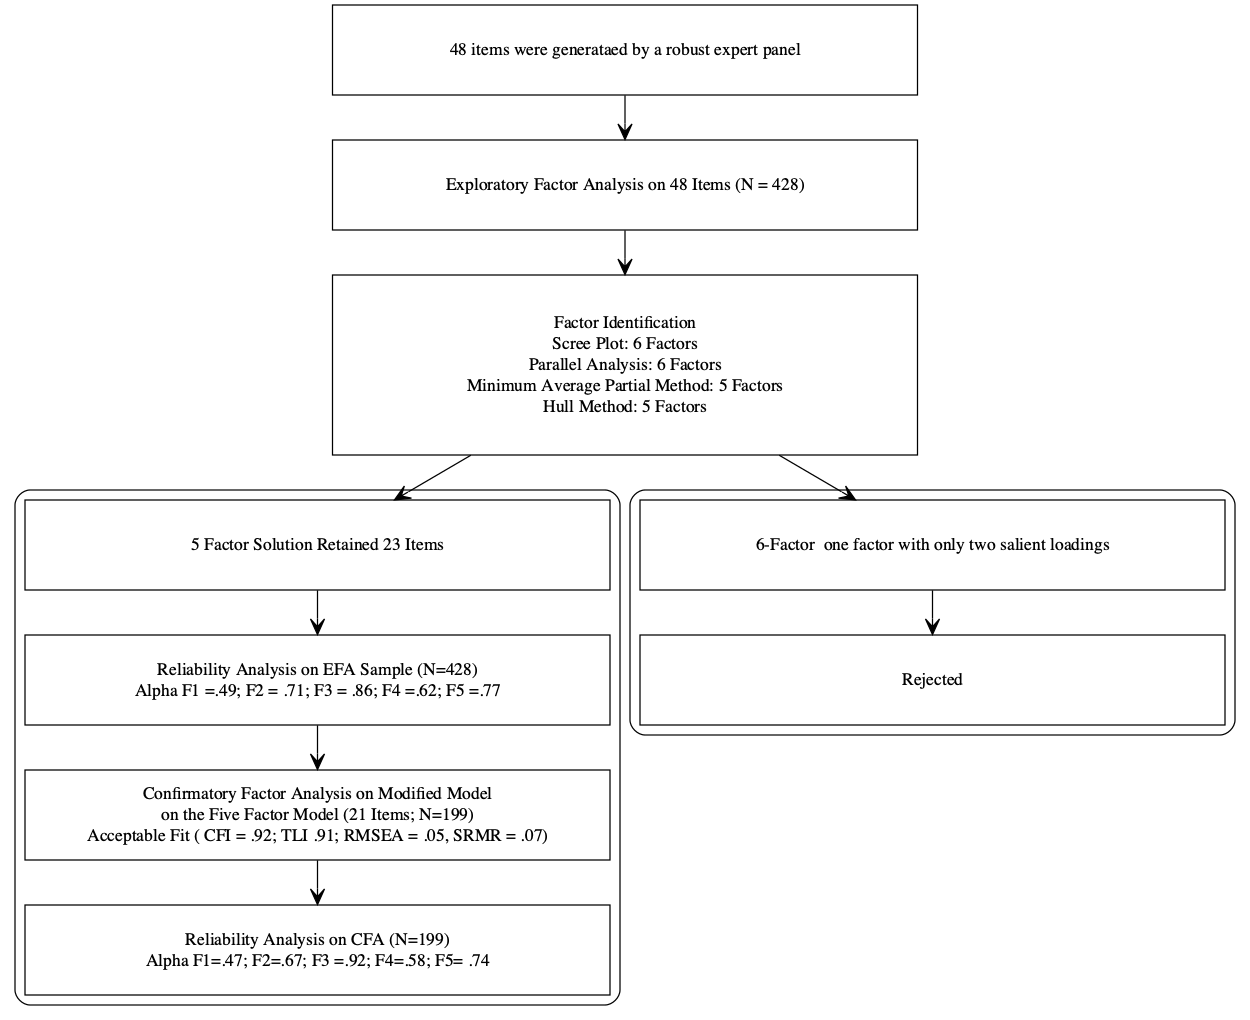
\includegraphics[width=4.17in,height=0.5\textheight]{Flowchart1} 

}

\caption{ABC}\label{fig:unnamed-chunk-1}
\end{figure}

\hypertarget{procedure}{%
\subsection{Procedure}\label{procedure}}

Our study had four objectives. First, to develop an instrument to assess individual's light exposure behavior . Second, to conduct an exploratory factor analysis(EFA) to understand the latent structure. Third to gather structural validity evidence for the latent structure obtained in EFA (Furr, 2014). Lastly, we gathered item information using Item response theory (IRT)(Baker, 2017)

\hypertarget{data-collection}{%
\subsubsection{Data Collection}\label{data-collection}}

Timeline of data collection, ethical approval, mode of data collection, how consent was recorded.

\hypertarget{item-generation-and-content-validity-expert-panel-review}{%
\subsubsection{Item generation and Content Validity: Expert Panel Review}\label{item-generation-and-content-validity-expert-panel-review}}

How we developed the 48 items?

\hypertarget{analytic-strategies}{%
\subsection{Analytic Strategies}\label{analytic-strategies}}

We used R (version 4.1.0), including several R-packages for our analyses. Necessary assumptions of EFA, including sample adequacy, normality assumptions, quality of correlation matrix were assessed. Our data violated both the univariate and multivariate normality assumptions. Due to these violations and the ordinal nature of our response data we used polychoric correlation matrix (Desjardins \& Bulut, 2018) for the EFA. We employed principal axis (pa) a factor extraction method with varimax rotation. PA is apparently robust to the normality assumption violations (Watkins, 2020). The obtained latent structure was confirmed by weighted least squares (WLS) extraction method as well. We used a combination factor indentification method including scree plot(Cattell, 1966), Horn's parallel analysis (Horn, 1965), minimum average partials method(Velicer, 1976), and hull method (Lorenzo-Seva, Timmerman, \& Kiers, 2011) to identify factor numbers. Additionally, to identify the simple structure we followed the following guidelines recommended by psychometricians (i) no factors with fewer than three items (ii) no factors with a factor loading \textless0.3 (iii) no items with cross-loading greater than .3 across factors (Bandalos \& Finney, 2018; Child, 2006; Mulaik, 2009; Watkins, 2020)

\hypertarget{results}{%
\section{Results}\label{results}}

Sampling adequacy was investigated by Kaiser-Meyer-Olkin (KMO) measures of sampling adequacy(Kaiser, 1974) . The overall KMO vale for 23 items was 0.63 which was above the cutoff value of .50 indicating a mediocre sample (Hutcheson, 1999).

\begin{table}[tbp]

\begin{center}
\begin{threeparttable}

\caption{\label{tab:tabDes}Descriptive Statistics}

\begin{tabular}{llllllll}
\toprule
 & \multicolumn{1}{c}{Mean} & \multicolumn{1}{c}{SD} & \multicolumn{1}{c}{Skew} & \multicolumn{1}{c}{Kurtosis} & \multicolumn{1}{c}{Shapiro-Wilk Statistics} & \multicolumn{1}{c}{p} & \multicolumn{1}{c}{Item-Total Correlation}\\
\midrule
Item1 & 1.12 & 0.49 & 5.02 & 27.80 & 0.25 & .00 & .16\\
Item2 & 2.16 & 1.19 & 0.71 & -0.54 & 0.84 & .00 & .14\\
Item3 & 4.14 & 0.99 & -1.23 & 1.14 & 0.79 & .00 & .19\\
Item4 & 2.87 & 1.59 & 0.08 & -1.60 & 0.83 & .00 & .19\\
Item5 & 1.76 & 1.23 & 1.35 & 0.44 & 0.66 & .00 & .38\\
Item6 & 2.73 & 1.46 & 0.20 & -1.36 & 0.87 & .00 & .33\\
Item7 & 3.86 & 1.67 & -0.99 & -0.85 & 0.65 & .00 & .23\\
Item8 & 3.76 & 1.14 & -0.68 & -0.45 & 0.86 & .00 & .00\\
Item9 & 3.42 & 1.83 & -0.45 & -1.69 & 0.69 & .00 & .33\\
Item10 & 2.74 & 1.04 & 0.09 & -0.74 & 0.91 & .00 & .28\\
Item11 & 2.60 & 1.25 & 0.29 & -0.86 & 0.89 & .00 & .35\\
Item12 & 2.11 & 1.17 & 0.77 & -0.39 & 0.83 & .00 & .32\\
Item13 & 2.94 & 1.03 & -0.12 & -0.40 & 0.91 & .00 & .10\\
Item14 & 3.62 & 1.64 & -0.68 & -1.25 & 0.74 & .00 & .32\\
Item15 & 1.64 & 1.18 & 1.79 & 2.02 & 0.60 & .00 & .15\\
Item16 & 3.51 & 1.30 & -0.70 & -0.59 & 0.85 & .00 & .39\\
Item17 & 1.96 & 0.98 & 1.02 & 0.69 & 0.82 & .00 & .05\\
Item18 & 2.44 & 1.31 & 0.38 & -1.14 & 0.86 & .00 & .11\\
Item19 & 3.80 & 1.29 & -0.87 & -0.42 & 0.82 & .00 & .17\\
Item20 & 4.01 & 1.40 & -1.22 & 0.07 & 0.70 & .00 & .13\\
Item21 & 1.33 & 0.91 & 3.03 & 8.43 & 0.41 & .00 & .01\\
Item22 & 2.59 & 1.41 & 0.27 & -1.27 & 0.86 & .00 & .19\\
Item23 & 1.31 & 0.81 & 2.75 & 6.92 & 0.43 & .00 & .21\\
Item24 & 1.47 & 1.18 & 2.38 & 4.00 & 0.43 & .00 & .28\\
Item25 & 2.56 & 1.27 & 0.33 & -1.00 & 0.89 & .00 & .11\\
Item26 & 1.54 & 1.25 & 2.13 & 2.86 & 0.46 & .00 & .36\\
Item27 & 4.30 & 1.08 & -1.79 & 2.53 & 0.67 & .00 & .22\\
Item28 & 2.27 & 1.39 & 0.74 & -0.81 & 0.81 & .00 & .25\\
Item29 & 3.26 & 1.09 & -0.26 & -0.45 & 0.91 & .00 & .14\\
Item30 & 2.22 & 1.48 & 0.71 & -1.02 & 0.76 & .00 & .30\\
Item31 & 1.05 & 0.36 & 7.23 & 52.98 & 0.13 & .00 & .18\\
Item32 & 1.54 & 1.21 & 2.07 & 2.75 & 0.49 & .00 & .31\\
Item33 & 1.04 & 0.33 & 8.99 & 85.28 & 0.10 & .00 & .16\\
Item34 & 3.36 & 1.38 & -0.48 & -1.03 & 0.87 & .00 & .16\\
Item35 & 2.26 & 1.25 & 0.70 & -0.60 & 0.85 & .00 & .19\\
Item36 & 2.36 & 1.22 & 0.59 & -0.62 & 0.87 & .00 & .25\\
Item37 & 1.14 & 0.59 & 4.79 & 24.05 & 0.25 & .00 & .16\\
Item38 & 2.25 & 1.27 & 0.69 & -0.64 & 0.84 & .00 & .18\\
Item39 & 3.93 & 1.48 & -1.06 & -0.44 & 0.71 & .00 & .18\\
Item40 & 3.57 & 1.07 & -0.65 & -0.17 & 0.88 & .00 & .21\\
Item41 & 3.55 & 1.65 & -0.60 & -1.34 & 0.76 & .00 & .43\\
Item42 & 3.00 & 1.62 & -0.08 & -1.61 & 0.83 & .00 & .44\\
Item43 & 1.56 & 1.23 & 2.00 & 2.45 & 0.50 & .00 & .32\\
Item44 & 2.97 & 1.20 & -0.06 & -0.94 & 0.91 & .00 & -.10\\
Item45 & 2.79 & 1.55 & 0.19 & -1.48 & 0.85 & .00 & .20\\
Item46 & 2.14 & 1.31 & 0.77 & -0.78 & 0.80 & .00 & .26\\
Item47 & 2.18 & 0.90 & 0.60 & 0.12 & 0.86 & .00 & .26\\
Item48 & 1.48 & 1.11 & 2.18 & 3.35 & 0.48 & .00 & .24\\
\bottomrule
\end{tabular}

\end{threeparttable}
\end{center}

\end{table}

\begin{figure}
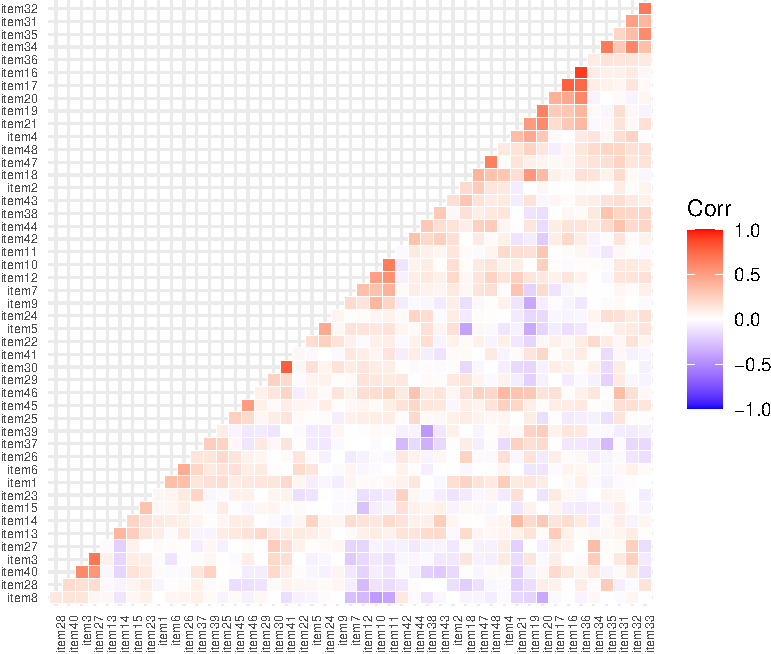
\includegraphics[width=0.5\linewidth]{manuscript_files/figure-latex/figCor-1} \caption{Iter-correlation of the items}\label{fig:figCor}
\end{figure}

Table\ref{tab:tabDes} summarizes the univariate descriptive statistics for the 48 items. some of the items were skewed with high Kurtosis values. The Shapiro-Wilk test of normality (Shapiro \& Wilk, 1965) indicated all the items violated normality assumptions. Multivariate normality assumptions were investigated by Marida's test (Mardia, 1970). Multivariate skew = 583.80 (p \textless0.001) and multivariate kurtosis = 2,749.15 (p \textless0.001) indicated multivariate normality assumptions violation. Due to these violations and ordinal nature of the response data polychoric correlations over Pearson's correlations was chosen (Desjardins \& Bulut, 2018). Bartlett's test of sphericity (Bartlett, 1954), \(\chi^2\) (1128) = 5042.86, p \textless{} .001{]} indicated the correlations between items are adequate for the EFA. However only 4.96\% of the inter-item correlation coefficients were greater than .30 in the obtained matrix. The inter item correlation ranged between .44 to .91. The corrected item-total correlations ranged between .10 to .44.

Scree plot ( Fig@ref(fig:fac.id)) suggested a six-factor solution.Horn's parallel analysis (Horn, 1965), like the Monte Carlo study, draws several sets of random data with the same number of participants as the original data set and compares the mean eigenvalues among the simulated and original data sets to retain optimal factors.This extraction method also supported a five-factor model. In our data set parallel analysis with 500 iterations indicated six-factor solution. However, In MAP method (Velicer, 1976) and Hull method (Lorenzo-Seva, Timmerman, \& Kiers, 2011) suggested a five-factor solution. As a result, we tested both five factor and six factor solutions. The histogram of the absolute values of non-redundant residual-correlations the proportion of non-redundant residual correlations greater than the absolute value of .05 should be small

\begin{figure}

{\centering 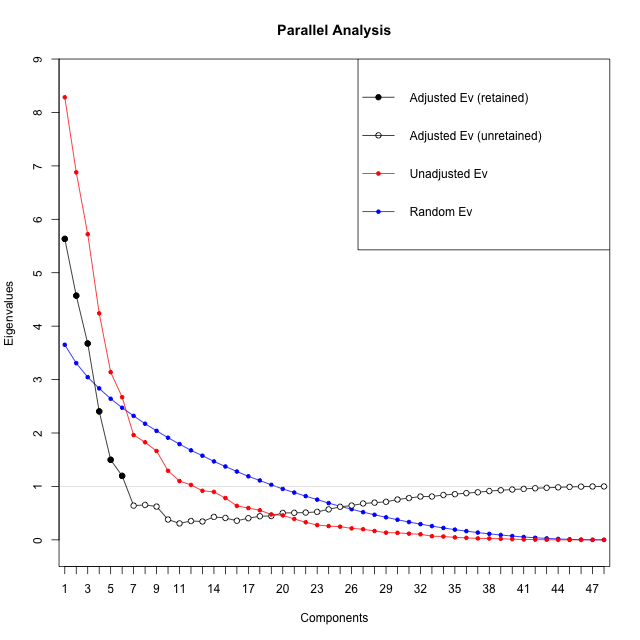
\includegraphics[width=0.5\linewidth,height=0.5\textheight]{parallel} 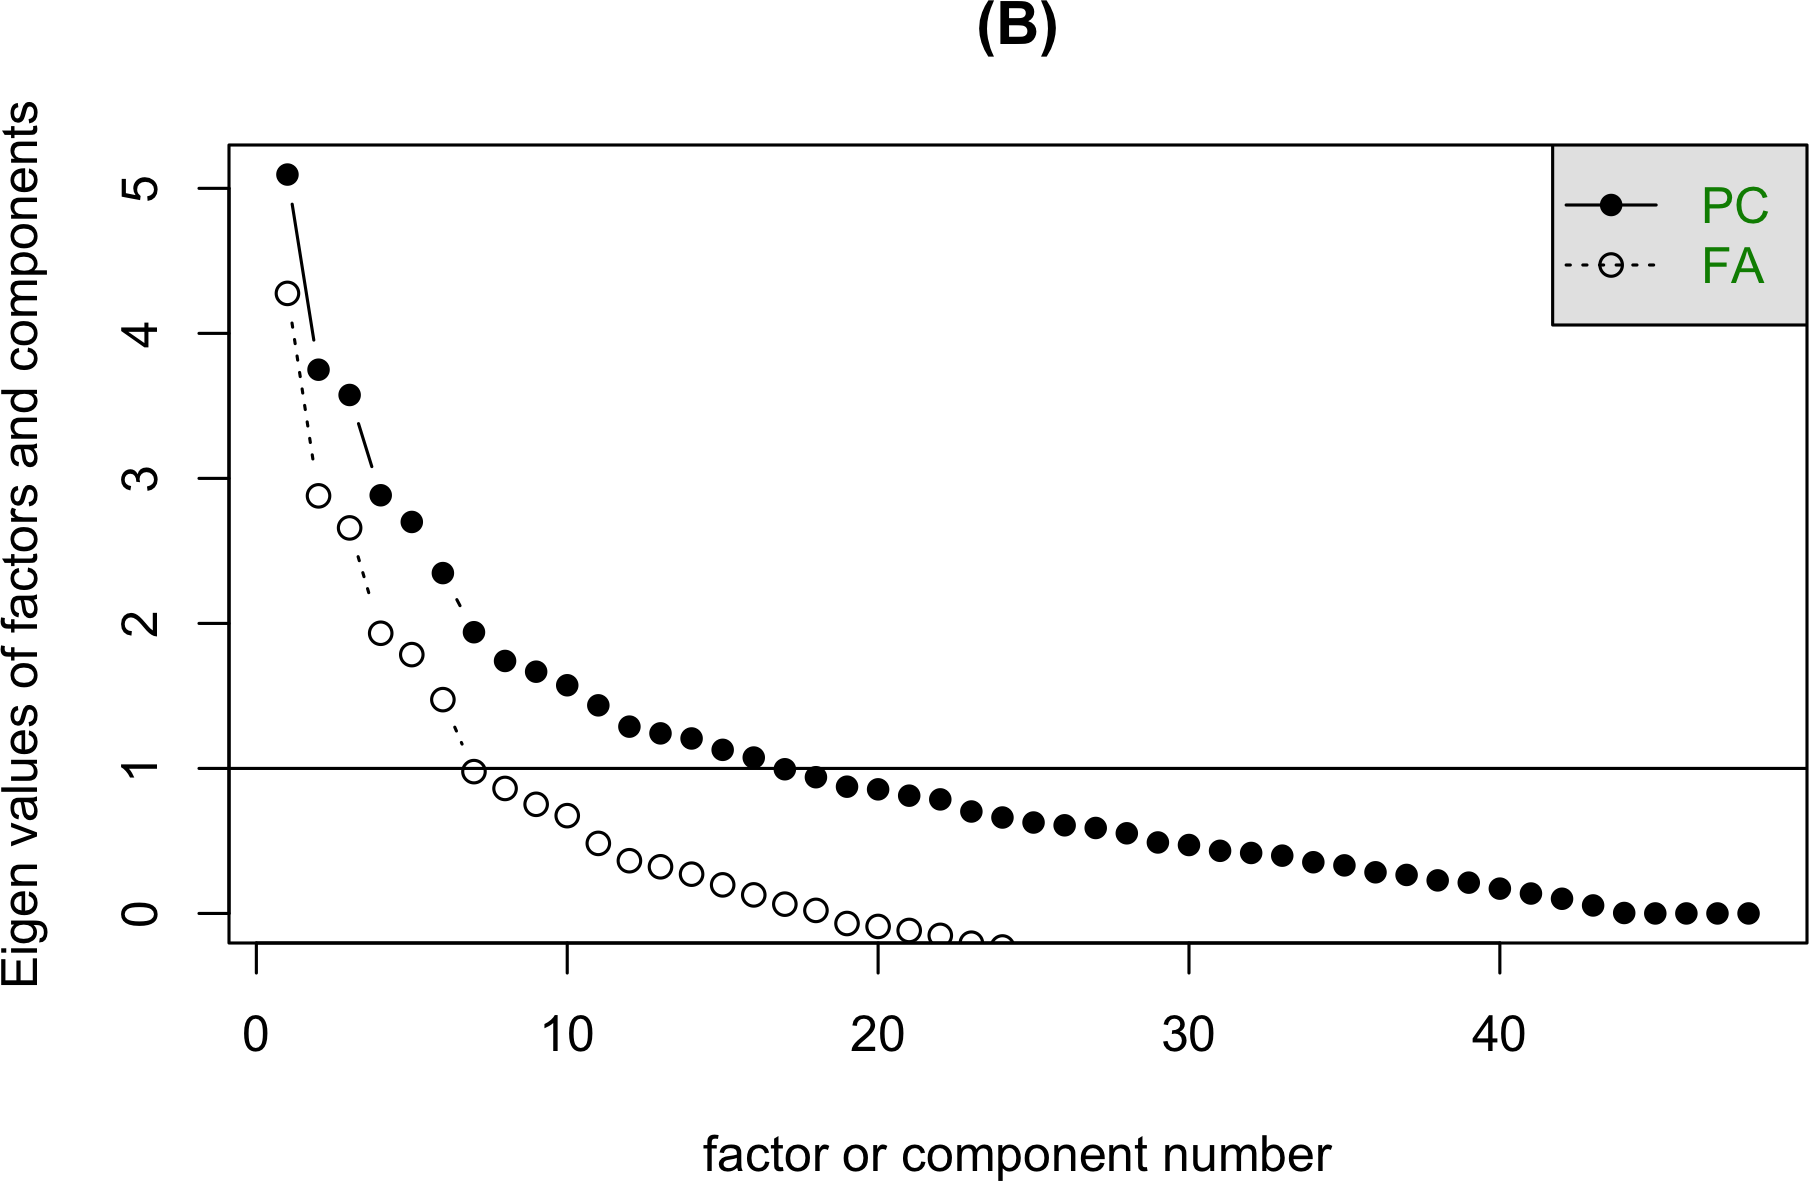
\includegraphics[width=0.5\linewidth,height=0.5\textheight]{manuscript_files/figure-latex/fac.id-2} 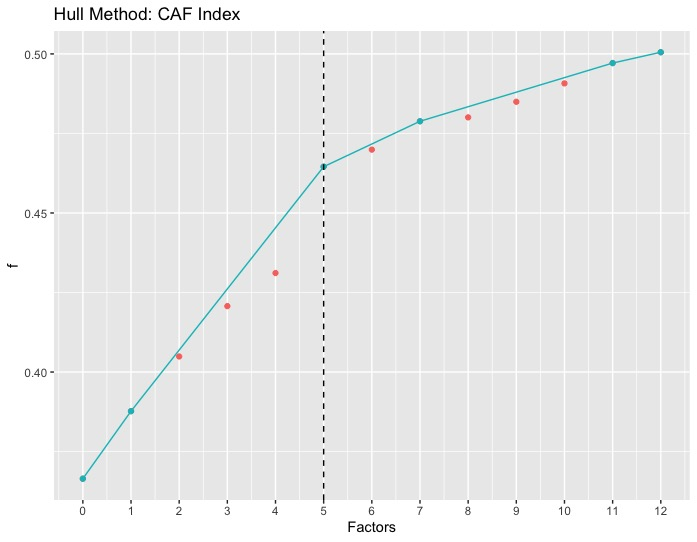
\includegraphics[width=0.5\linewidth,height=0.5\textheight]{HUll method} 

}

\caption{Factor Identification (A) Parallel analysis (B) Scree Plot, (C) Hull method}(\#fig:fac.id)
\end{figure}

\begin{table}[tbp]

\begin{center}
\begin{threeparttable}

\caption{\label{tab:TabEFA5}}

\begin{tabular}{lllllll}
\toprule
 & \multicolumn{1}{c}{F1} & \multicolumn{1}{c}{F2} & \multicolumn{1}{c}{F3} & \multicolumn{1}{c}{F4} & \multicolumn{1}{c}{F5} & \multicolumn{1}{c}{Communalities}\\
\midrule
item1 & 0.06 & -0.03 & 0.01 & 0.03 & 0.35 & 0.13\\
item2 & 0.12 & -0.10 & -0.11 & 0.69 & -0.03 & 0.51\\
item5 & 0.01 & 0.16 & 0.09 & 0.01 & 0.69 & 0.52\\
item7 & 0.06 & -0.09 & 0.66 & -0.01 & -0.03 & 0.45\\
item10 & -0.01 & 0.82 & 0.07 & 0.02 & 0.02 & 0.68\\
item13 & -0.06 & 0.34 & -0.03 & 0.10 & 0.00 & 0.13\\
item14 & 0.00 & 0.05 & 0.89 & -0.08 & -0.08 & 0.81\\
item16 & 0.10 & 0.05 & 0.29 & -0.11 & 0.31 & 0.21\\
item19 & 0.02 & -0.06 & 0.00 & 0.80 & 0.03 & 0.64\\
item21 & -0.05 & -0.02 & -0.34 & 0.03 & -0.06 & 0.12\\
item24 & -0.03 & 0.10 & 0.10 & 0.11 & 0.54 & 0.33\\
item26 & 0.93 & 0.00 & 0.13 & -0.01 & 0.13 & 0.90\\
item27 & -0.01 & 0.07 & 0.38 & -0.12 & 0.21 & 0.21\\
item28 & 0.02 & 0.00 & -0.05 & 0.01 & 0.31 & 0.10\\
item30 & 0.06 & 0.01 & 0.11 & -0.04 & 0.52 & 0.29\\
item32 & 0.80 & 0.00 & 0.05 & 0.13 & 0.10 & 0.67\\
item34 & -0.01 & -0.14 & 0.02 & 0.84 & 0.12 & 0.74\\
item35 & -0.04 & 0.46 & 0.04 & -0.17 & 0.04 & 0.25\\
item36 & 0.09 & 0.63 & 0.10 & -0.15 & 0.11 & 0.45\\
item41 & 0.05 & 0.07 & 0.70 & 0.30 & 0.14 & 0.60\\
item43 & 0.99 & 0.00 & 0.06 & 0.01 & 0.03 & 0.99\\
item44 & -0.03 & -0.47 & -0.01 & 0.10 & 0.01 & 0.24\\
item47 & 0.02 & 0.82 & -0.05 & -0.06 & 0.16 & 0.70\\
\bottomrule
\end{tabular}

\end{threeparttable}
\end{center}

\end{table}

The initial five-factor solution with all 48 items showed the presence of cross-loading items (item 42, 16, \& 1) and poor factor loading (\textless.30) items (item 20,3 ,15, 17, 40, 4, 11, 39, 18, 45, 29, 25, 8 , \& 46). At first we discard the items with poor factor loading and ran another EFA on the remaining 34 items. This iteration of EFA also appeared as a misfit in terms of poor factor loading (Item 12, 22, 38, 6) and cross-loading (items 23, 31, 37, 48) . Another two rounds of EFA were conducted with gradually identifying problematic items and discarding them from the model. Finally, a five-factor EFA solution with 23 items was accepted with RMSR = 0.04, no loading smaller than .30 and no cross-loading greater than .30.

\begin{figure}

{\centering \includegraphics[height=0.5\textheight]{manuscript_files/figure-latex/FivRes-1} 

}

\caption{ Residulas of five-dactor solution}\label{fig:FivRes}
\end{figure}

\hypertarget{confirmatory-factor-analysis}{%
\section{Confirmatory Factor Analysis}\label{confirmatory-factor-analysis}}

\hypertarget{discussion}{%
\section{Discussion}\label{discussion}}

\newpage

\hypertarget{references}{%
\section{References}\label{references}}

\begingroup
\setlength{\parindent}{-0.5in}
\setlength{\leftskip}{0.5in}

\hypertarget{refs}{}
\begin{CSLReferences}{1}{0}
\leavevmode\hypertarget{ref-R-papaja}{}%
Aust, F., \& Barth, M. (2020). \emph{{papaja}: {Prepare} reproducible {APA} journal articles with {R Markdown}}. Retrieved from \url{https://github.com/crsh/papaja}

\leavevmode\hypertarget{ref-bakerBasicsItemResponse2017}{}%
Baker, F. B. (2017). \emph{The {Basics} of {Item Response Theory Using R}} (1st ed. 2017.). {Springer}.

\leavevmode\hypertarget{ref-bandalosFactorAnalysisExploratory2018}{}%
Bandalos, D. L., \& Finney, S. J. (2018). Factor analysis: {Exploratory} and confirmatory. In \emph{The reviewer's guide to quantitative methods in the social sciences} (pp. 98--122). {Routledge}.

\leavevmode\hypertarget{ref-R-tinylabels}{}%
Barth, M. (2021). \emph{{tinylabels}: Lightweight variable labels}. Retrieved from \url{https://github.com/mariusbarth/tinylabels}

\leavevmode\hypertarget{ref-bartlettNoteMultiplyingFactors1954}{}%
Bartlett, M. (1954). A {Note} on the {Multiplying Factors} for {Various Chi}-square {Approximations}. \emph{Journal of the Royal Statistical Society. Series B, Methodological}, \emph{16}(2), 296--298.

\leavevmode\hypertarget{ref-R-MOTE}{}%
Buchanan, E. M., Gillenwaters, A., Scofield, J. E., \& Valentine, K. D. (2019). \emph{{MOTE: Measure of the Effect}: Package to assist in effect size calculations and their confidence intervals}. Retrieved from \url{http://github.com/doomlab/MOTE}

\leavevmode\hypertarget{ref-cattellScreeTestNumber1966}{}%
Cattell, R. B. (1966). The {Scree Test For The Number Of Factors}. \emph{Multivariate Behavioral Research}, \emph{1}(2), 245--276. \url{https://doi.org/10.1207/s15327906mbr0102_10}

\leavevmode\hypertarget{ref-R-shiny}{}%
Chang, W., Cheng, J., Allaire, J., Sievert, C., Schloerke, B., Xie, Y., \ldots{} Borges, B. (2021). \emph{Shiny: Web application framework for r}. Retrieved from \url{https://CRAN.R-project.org/package=shiny}

\leavevmode\hypertarget{ref-childEssentialsFactorAnalysis2006}{}%
Child, D. (2006). \emph{Essentials of factor analysis} (3rd ed.). {New York: Continuum}.

\leavevmode\hypertarget{ref-desjardinsHandbookEducationalMeasurement2018}{}%
Desjardins, C., \& Bulut, O. (2018). \emph{Handbook of {Educational Measurement} and {Psychometrics Using R}}. \url{https://doi.org/10.1201/b20498}

\leavevmode\hypertarget{ref-R-paran}{}%
Dinno, A. (2018). \emph{Paran: Horn's test of principal components/factors}. Retrieved from \url{https://CRAN.R-project.org/package=paran}

\leavevmode\hypertarget{ref-R-semPlot}{}%
Epskamp, S. (2019). \emph{semPlot: Path diagrams and visual analysis of various SEM packages' output}. Retrieved from \url{https://CRAN.R-project.org/package=semPlot}

\leavevmode\hypertarget{ref-R-qgraph}{}%
Epskamp, S., Cramer, A. O. J., Waldorp, L. J., Schmittmann, V. D., \& Borsboom, D. (2012). {qgraph}: Network visualizations of relationships in psychometric data. \emph{Journal of Statistical Software}, \emph{48}(4), 1--18.

\leavevmode\hypertarget{ref-furrPsychometricsIntroduction2014}{}%
Furr, R. M. (2014). \emph{Psychometrics : An introduction} (2nd ed.). {Thousand Oaks}: {Thousand Oaks : SAGE}.

\leavevmode\hypertarget{ref-R-purrr}{}%
Henry, L., \& Wickham, H. (2020). \emph{Purrr: Functional programming tools}. Retrieved from \url{https://CRAN.R-project.org/package=purrr}

\leavevmode\hypertarget{ref-hornRationaleTestNumber1965}{}%
Horn, J. L. (1965). A rationale and test for the number of factors in factor analysis. \emph{Psychometrika}, \emph{30}(2), 179--185. \url{https://doi.org/10.1007/BF02289447}

\leavevmode\hypertarget{ref-hutchesonMultivariateSocialScientist1999}{}%
Hutcheson, G. D. (1999). \emph{The multivariate social scientist : Introductory statistics using generalized linear models}. {London : SAGE}.

\leavevmode\hypertarget{ref-R-DiagrammeRsvg}{}%
Iannone, R. (2016). \emph{DiagrammeRsvg: Export DiagrammeR graphviz graphs as SVG}. Retrieved from \url{https://CRAN.R-project.org/package=DiagrammeRsvg}

\leavevmode\hypertarget{ref-R-DiagrammeR}{}%
Iannone, R. (2021). \emph{DiagrammeR: Graph/network visualization}. Retrieved from \url{https://github.com/rich-iannone/DiagrammeR}

\leavevmode\hypertarget{ref-R-semTools}{}%
Jorgensen, T. D., Pornprasertmanit, S., Schoemann, A. M., \& Rosseel, Y. (2021). \emph{\texttt{semTools}: {U}seful tools for structural equation modeling}. Retrieved from \url{https://CRAN.R-project.org/package=semTools}

\leavevmode\hypertarget{ref-kaiserIndexFactorialSimplicity1974}{}%
Kaiser, H. F. (1974). An index of factorial simplicity. \emph{Psychometrika}, \emph{39}(1), 31--36. \url{https://doi.org/10.1007/bf02291575}

\leavevmode\hypertarget{ref-lorenzo-sevaHullMethodSelecting2011}{}%
Lorenzo-Seva, U., Timmerman, M., \& Kiers, H. (2011). The {Hull Method} for {Selecting} the {Number} of {Common Factors}. \emph{Multivariate Behavioral Research}, \emph{46}, 340--364. \url{https://doi.org/10.1080/00273171.2011.564527}

\leavevmode\hypertarget{ref-mardiaMeasuresMultivariateSkewness1970}{}%
Mardia, K. V. (1970). Measures of multivariate skewness and kurtosis with applications. \emph{Biometrika}, \emph{57}(3), 519--530. \url{https://doi.org/10.1093/biomet/57.3.519}

\leavevmode\hypertarget{ref-mulaikFoundationsFactorAnalysis2009}{}%
Mulaik, S. A. (2009). \emph{Foundations of {Factor Analysis}} (Vol. 7). {London}: {London: Chapman and Hall/CRC}. \url{https://doi.org/10.1201/b15851}

\leavevmode\hypertarget{ref-R-tibble}{}%
Müller, K., \& Wickham, H. (2021). \emph{Tibble: Simple data frames}. Retrieved from \url{https://CRAN.R-project.org/package=tibble}

\leavevmode\hypertarget{ref-R-EFA.MRFA}{}%
Navarro-Gonzalez, D., \& Lorenzo-Seva, U. (2021). \emph{EFA.MRFA: Dimensionality assessment using minimum rank factor analysis}. Retrieved from \url{https://CRAN.R-project.org/package=EFA.MRFA}

\leavevmode\hypertarget{ref-R-rsvg}{}%
Ooms, J. (2021). \emph{Rsvg: Render SVG images into PDF, PNG, PostScript, or bitmap arrays}. Retrieved from \url{https://CRAN.R-project.org/package=rsvg}

\leavevmode\hypertarget{ref-R-base}{}%
R Core Team. (2021). \emph{R: A language and environment for statistical computing}. Vienna, Austria: R Foundation for Statistical Computing. Retrieved from \url{https://www.R-project.org/}

\leavevmode\hypertarget{ref-R-psych}{}%
Revelle, W. (2021). \emph{Psych: Procedures for psychological, psychometric, and personality research}. Evanston, Illinois: Northwestern University. Retrieved from \url{https://CRAN.R-project.org/package=psych}

\leavevmode\hypertarget{ref-R-lavaan}{}%
Rosseel, Y. (2012). {lavaan}: An {R} package for structural equation modeling. \emph{Journal of Statistical Software}, \emph{48}(2), 1--36. Retrieved from \url{https://www.jstatsoft.org/v48/i02/}

\leavevmode\hypertarget{ref-R-dlookr}{}%
Ryu, C. (2021). \emph{Dlookr: Tools for data diagnosis, exploration, transformation}. Retrieved from \url{https://CRAN.R-project.org/package=dlookr}

\leavevmode\hypertarget{ref-shapiroAnalysisVarianceTest1965}{}%
Shapiro, S. S., \& Wilk, M. B. (1965). An analysis of variance test for normality (complete samples). \emph{Biometrika}, \emph{52}(3-4), 591--611. \url{https://doi.org/10.1093/biomet/52.3-4.591}

\leavevmode\hypertarget{ref-velicerDeterminingNumberComponents1976}{}%
Velicer, W. (1976). Determining the {Number} of {Components} from the {Matrix} of {Partial Correlations}. \emph{Psychometrika}, \emph{41}, 321--327. \url{https://doi.org/10.1007/BF02293557}

\leavevmode\hypertarget{ref-R-MASS}{}%
Venables, W. N., \& Ripley, B. D. (2002). \emph{Modern applied statistics with s} (Fourth). New York: Springer. Retrieved from \url{https://www.stats.ox.ac.uk/pub/MASS4/}

\leavevmode\hypertarget{ref-watkinsStepbyStepGuideExploratory2020}{}%
Watkins, M. (2020). \emph{A {Step}-by-{Step Guide} to {Exploratory Factor Analysis} with {R} and {RStudio}}. \url{https://doi.org/10.4324/9781003120001}

\leavevmode\hypertarget{ref-R-ggplot2}{}%
Wickham, H. (2016). \emph{ggplot2: Elegant graphics for data analysis}. Springer-Verlag New York. Retrieved from \url{https://ggplot2.tidyverse.org}

\leavevmode\hypertarget{ref-R-stringr}{}%
Wickham, H. (2019). \emph{Stringr: Simple, consistent wrappers for common string operations}. Retrieved from \url{https://CRAN.R-project.org/package=stringr}

\leavevmode\hypertarget{ref-R-forcats}{}%
Wickham, H. (2021a). \emph{Forcats: Tools for working with categorical variables (factors)}. Retrieved from \url{https://CRAN.R-project.org/package=forcats}

\leavevmode\hypertarget{ref-R-tidyr}{}%
Wickham, H. (2021b). \emph{Tidyr: Tidy messy data}. Retrieved from \url{https://CRAN.R-project.org/package=tidyr}

\leavevmode\hypertarget{ref-R-tidyverse}{}%
Wickham, H., Averick, M., Bryan, J., Chang, W., McGowan, L. D., François, R., \ldots{} Yutani, H. (2019). Welcome to the {tidyverse}. \emph{Journal of Open Source Software}, \emph{4}(43), 1686. \url{https://doi.org/10.21105/joss.01686}

\leavevmode\hypertarget{ref-R-readxl}{}%
Wickham, H., \& Bryan, J. (2019). \emph{Readxl: Read excel files}. Retrieved from \url{https://CRAN.R-project.org/package=readxl}

\leavevmode\hypertarget{ref-R-dplyr}{}%
Wickham, H., François, R., Henry, L., \& Müller, K. (2021). \emph{Dplyr: A grammar of data manipulation}. Retrieved from \url{https://CRAN.R-project.org/package=dplyr}

\leavevmode\hypertarget{ref-R-readr}{}%
Wickham, H., \& Hester, J. (2021). \emph{Readr: Read rectangular text data}. Retrieved from \url{https://CRAN.R-project.org/package=readr}

\leavevmode\hypertarget{ref-R-kableExtra}{}%
Zhu, H. (2021). \emph{kableExtra: Construct complex table with 'kable' and pipe syntax}. Retrieved from \url{https://CRAN.R-project.org/package=kableExtra}

\end{CSLReferences}

\endgroup


\end{document}
